\documentclass[11pt,a4paper]{article}
\usepackage[utf8]{inputenc}
\usepackage[T1]{fontenc}
\usepackage{tgpagella}
\usepackage[spanish]{babel}
\usepackage{geometry}
\usepackage{booktabs}
\usepackage{xcolor}
\usepackage{titlesec}
\usepackage{fancyhdr}
\usepackage[parfill]{parskip}
\usepackage[expansion=false]{microtype}
\usepackage{hyperref}
\usepackage{setspace}
\usepackage{needspace}
\usepackage{graphicx}
\widowpenalty=10000
\clubpenalty=10000
\displaywidowpenalty=10000

\geometry{top=3.0cm,bottom=3.0cm,left=3.5cm,right=3.5cm}
\setlength{\parskip}{0.65em}
\setlength{\parindent}{0em}

\definecolor{azulai}{RGB}{30,80,140}
\definecolor{doradoai}{RGB}{140,90,0}
\definecolor{grisai}{RGB}{70,70,70}

\titleformat{\section}{\Large\bfseries\color{azulai}}{}{0em}{}[{\color{azulai}\titlerule[0.5pt]}]
\titlespacing*{\section}{0pt}{1.8em}{0.8em}
\titleformat{\subsection}{\large\bfseries\color{doradoai}}{}{0em}{}
\titlespacing*{\subsection}{0pt}{1.4em}{0.5em}
\titleformat{\subsubsection}{\normalsize\bfseries\color{grisai}}{}{0em}{}
\titlespacing*{\subsubsection}{0pt}{1.0em}{0.3em}

\pagestyle{fancy}\fancyhf{}
\rhead{\textcolor{grisai}{\small Maite Barragan — Arquitectura Interna}}
\lhead{\textcolor{grisai}{\small Sol · Ascendente · Nodos}}
\cfoot{\textcolor{grisai}{\small\thepage}}
\renewcommand{\headrulewidth}{0.3pt}

\hypersetup{colorlinks=true,linkcolor=azulai,urlcolor=azulai}
\setstretch{1.45}
\tolerance=1500
\emergencystretch=4em

\begin{document}

% ── Portada ──────────────────────────────────────────────────────────────────
\begin{titlepage}
  \centering
  \vspace*{1.5cm}
  {\Huge\bfseries\color{azulai} Sol · Ascendente · Nodos}\\[0.5cm]
  {\large\color{grisai} Arquitectura Interna}\\[0.3cm]
  {\small\itshape\color{grisai} Dirección vital, punto de entrada y eje de desarrollo}\\[2cm]
  {\huge\color{doradoai} Maite Barragan}\\[1.5cm]
  {\Large 07/01/1971 \quad 12:15}\\[0.3cm]
  {\Large Pamplona, España}\\[0.3cm]
  {\normalsize Lat: 42.8157° \quad Lon: -1.6522° \quad UTC+01:00}\\[0.3cm]
  {\normalsize Ascendente: Aries 6°18' \quad
    MC: Capricornio 3°11'}\\[2cm]
  \begin{tabular}{lll}
    \textbf{Sol:} & Capricornio & Casa 10 \\
    \textbf{Ascendente:} & Aries & Punto de entrada principal: Marte \\
    \textbf{Nodo Norte:} & Acuario & Casa 12 \\
    \textbf{Nodo Sur:}   & Leo & Casa 6 \\
  \end{tabular}\\[2cm]
  \vfill
  {\small Generado el 20/05/2026}
\end{titlepage}

\tableofcontents
\newpage

% ── Datos de referencia ───────────────────────────────────────────────────────
\section{Datos de referencia}

\begin{center}
\begin{tabular}{llll}
  \toprule
  \textbf{Punto} & \textbf{Signo} & \textbf{Casa} & \textbf{Posición} \\
  \midrule
  Sol           & Capricornio & 10 & 16°30' \\
  Ascendente    & Aries & --- & 6°18' \\
  Medio Cielo   & Capricornio & --- & 3°11' \\
  Nodo Norte    & Acuario & 12 & 24°17' \\
  Nodo Sur      & Leo & 6 & 24°17' \\
  \bottomrule
\end{tabular}
\end{center}

\vspace{0.5cm}
\textbf{Regente del Ascendente (Aries):} 
Marte —
Escorpio, 
Casa 8

\vspace{0.5cm}
\textbf{Aspectos entre Sol, Ascendente y Nodos:}

\vspace{0.3cm}
\textit{No aparecen aspectos directos entre Sol, Ascendente y Nodos dentro de los orbes definidos. Esto no significa ausencia de relación entre estos puntos, sino que la lectura se apoya principalmente en sus signos, casas, elementos e integración general.}

\needspace{3\baselineskip}
\subsection*{Grados sensibles}



\vspace{0.7cm}

\begin{center}
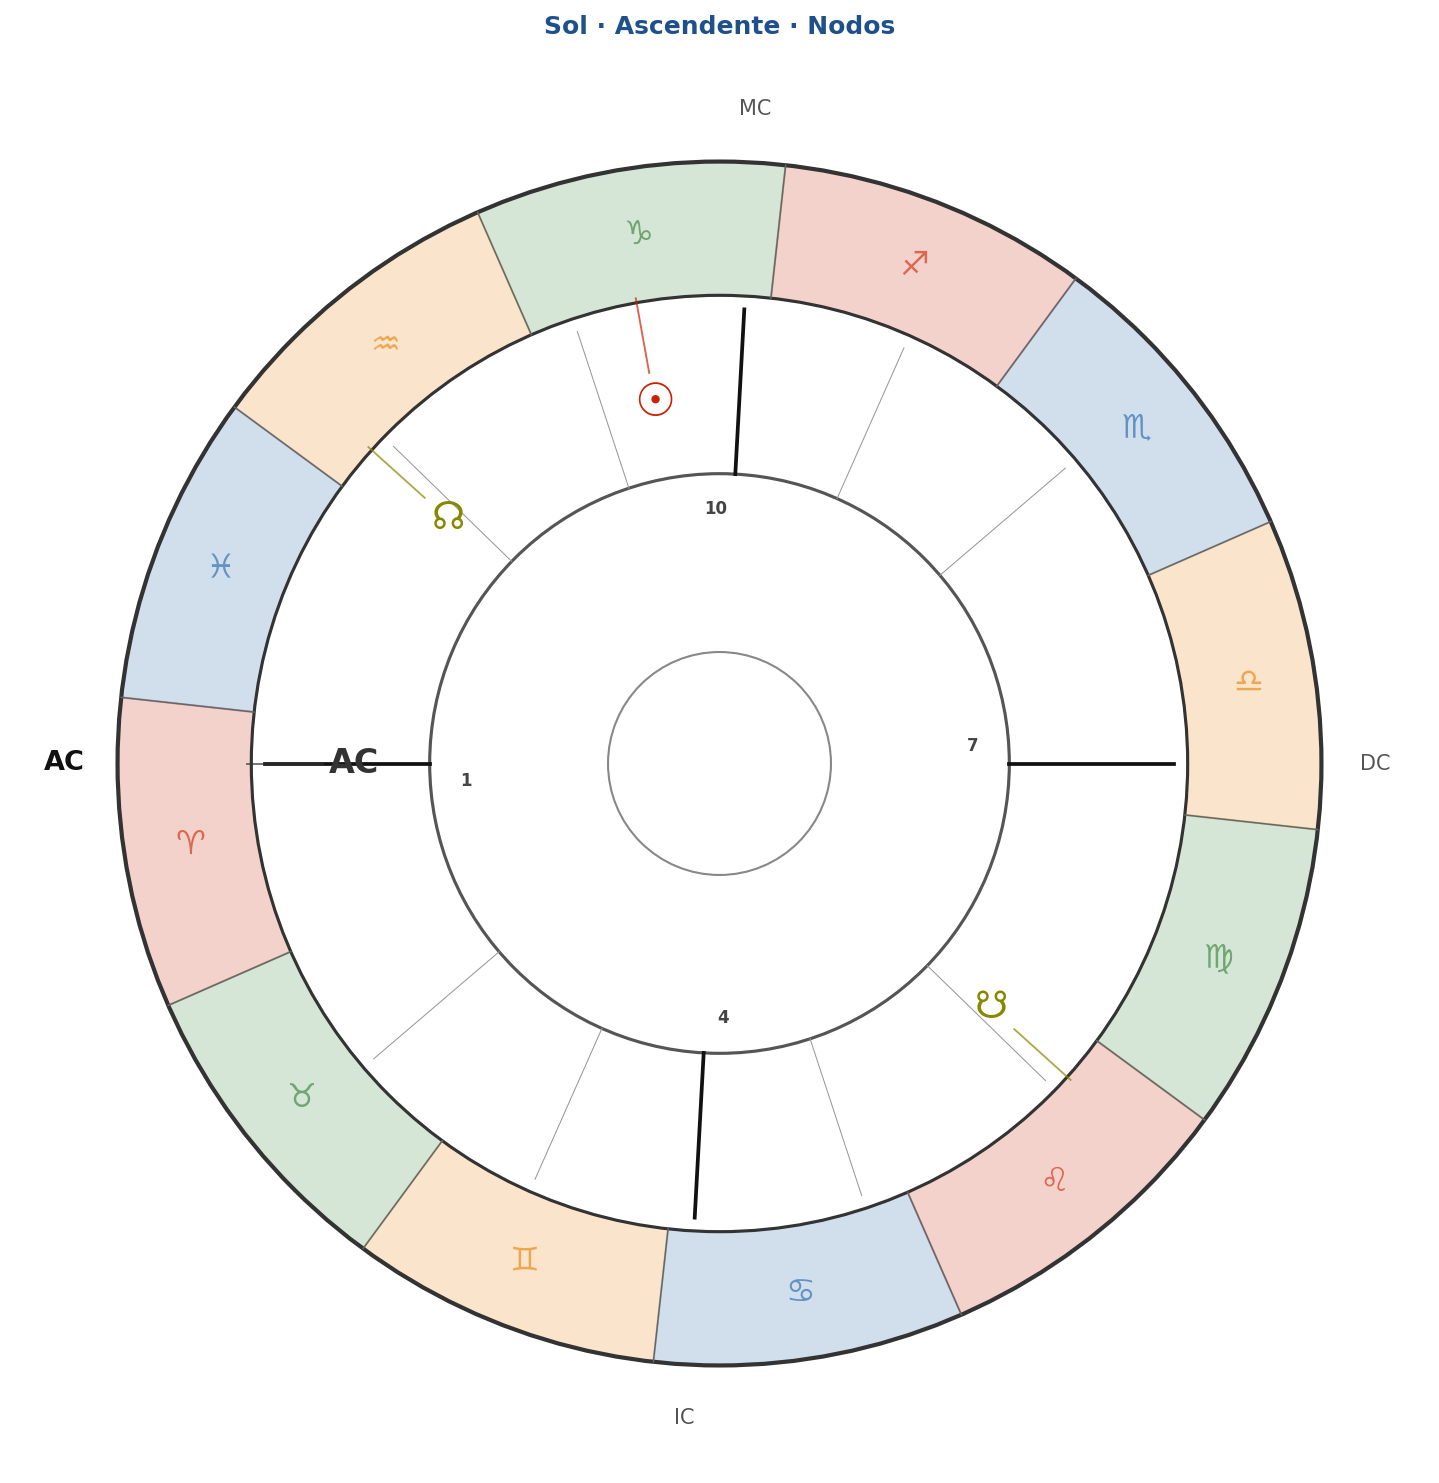
\includegraphics[width=0.72\textwidth]{Maite_Barragan_Sol_ASC_Nodos_rueda.png}
\end{center}


\vspace{0.3cm}
\Needspace{5\baselineskip}

% ── Interpretación ────────────────────────────────────────────────────────────
\section{Interpretación — Arquitectura Interna}

\begin{center}
{\small\itshape
No se trata de definir quién eres. Se trata de observar cómo se organiza tu dirección,
cómo atraviesas la vida y qué tensión influye en tu forma de avanzar.
}
\end{center}

\vspace{0.5cm}
\Needspace{5\baselineskip}


% ── 1. Dirección general ──────────────────────────────────────────────────────
\needspace{3\baselineskip}
\subsection{1. Dirección general}

El Sol está en Capricornio, Casa 10. El Ascendente está en Aries. El Nodo Norte está en Acuario, Casa 12, y el Nodo Sur en Leo, Casa 6.

El Sol en Capricornio y el Ascendente en Aries pertenecen a elementos con lógicas diferentes. Esto puede hacer que vivas las cosas de una forma, mientras otra parte de ti necesita orientarse desde un ritmo completamente diferente.

El Sol en Capricornio, Casa 10, no tiene un aspecto directo con los Nodos. La tensión entre el Nodo Norte en Acuario, Casa 12, y el Nodo Sur en Leo, Casa 6, se expresa de una forma más independiente respecto a la dirección solar.

\vspace{0.5cm}
\Needspace{5\baselineskip}


% ── 2. Sol ────────────────────────────────────────────────────────────────────
\needspace{3\baselineskip}
\subsection{2. El Sol — Dirección principal}

\needspace{3\baselineskip}
\subsubsection*{Sol en Capricornio · Casa 10}

Tu dirección se activa cuando puedes construir algo sólido a largo plazo. Necesitas objetivos claros, estructura y la sensación de que el esfuerzo actual servirá para algo en el futuro.

Sueles sostener bien procesos largos, pero te desgasta muchísimo trabajar sin dirección o invertir energía en cosas que no llevan a ningún lugar. La sensación de inutilidad puede agotarte más que el esfuerzo en sí.

Te afecta perder la estructura que organizaba tu vida, sentir que todo depende únicamente de ti o no ver resultados después de mucho tiempo sosteniendo algo. Necesitas sentir que estás construyendo sobre una base real.

Tu dirección se fortalece cuando puedes construir un lugar claro en el mundo. Necesitas sentir que avanzas hacia algo reconocible, sólido y con proyección.

Te afecta mucho no saber hacia dónde estás construyendo o sentir que todo el esfuerzo queda suspendido sin forma.

Sueles sostener bien las responsabilidades cuando tienen sentido para ti. La dirección aparece con más claridad cuando puedes asumir tu lugar y desarrollar una vocación propia.


\vspace{0.5cm}
\Needspace{5\baselineskip}


% ── 3. Ascendente ─────────────────────────────────────────────────────────────
\needspace{3\baselineskip}
\subsection{3. El Ascendente — Forma de relacionarte con la vida}

\needspace{3\baselineskip}
\subsubsection*{Aries · Regente: Marte}

Sueles vivir las cosas de forma rápida e inmediata. Muchas veces necesitas moverte, actuar o reaccionar para entender realmente lo que te está pasando.

Cuando pasas demasiado tiempo conteniéndote, esperando o sin poder actuar, es fácil que la tensión se acumule en el cuerpo. Puede aparecer irritación, impaciencia o una sensación constante de presión interna.

Te ayuda poder iniciar, probar, equivocarte y ajustar sobre la marcha. Cuando todo queda detenido durante demasiado tiempo, también se bloquea la forma en la que procesas lo que te ocurre.

El regente del Ascendente es Marte, situado en Escorpio, Casa 8. Marte pertenece a un elemento con una lógica diferente a la del Ascendente. Esto puede hacer que vivas las cosas de una forma, mientras otra parte de ti necesita orientarse desde un ritmo completamente diferente.. La Casa 8 muestra un territorio importante desde el que organizas tu forma de entrar en la vida.

\vspace{0.5cm}
\Needspace{5\baselineskip}


% ── 4. Nodos ──────────────────────────────────────────────────────────────────
\needspace{3\baselineskip}
\subsection{4. Nodo Norte y Nodo Sur — Dirección de crecimiento}

\needspace{3\baselineskip}
\subsubsection*{Nodo Norte en Acuario · Casa 12 \\
Nodo Sur en Leo · Casa 6}

Tu dirección pide ampliar la mirada y participar en algo que vaya más allá de lo puramente personal. Necesitas aprender a colaborar, compartir visión y construir también desde lo colectivo sin sentir que eso borra tu identidad. Lo conocido suele llevarte hacia la necesidad de reconocimiento individual o hacia la sensación de que todo depende exclusivamente de tu propia expresión personal. El reto está en contribuir sin necesitar constantemente confirmación externa sobre tu valor o tu importancia. Crecer hacia este Nodo Norte implica descubrir que formar parte de algo mayor no elimina lo que eres.

Tu dirección pide desarrollar más espacio interno, silencio y capacidad de escuchar procesos que no siempre pueden explicarse o resolverse rápidamente. El crecimiento aparece cuando aprendes a parar, descansar y permitir que algunas cosas maduren sin necesidad de controlarlas continuamente. El reto suele estar en no vivir permanentemente desde la hiperactividad, la exigencia o la necesidad de tener respuestas inmediatas para todo lo que ocurre.

Tiendes a buscar reconocimiento, centralidad o validación a través de lo que expresas y haces visible. Hay facilidad para crear, destacar y dejar una huella personal en lo que haces, pero también riesgo de depender demasiado de la mirada externa para sostener el propio valor. Puede aparecer necesidad constante de sentirte visto, importante o reconocido para confirmar que lo que haces tiene sentido. El problema surge cuando toda la experiencia empieza a girar alrededor de la validación externa o del lugar que ocupas frente a otras personas.

Tiendes a apoyarte en el control cotidiano, la organización y la necesidad de que todo funcione correctamente. Hay facilidad para sostener rutinas, resolver problemas y hacerte cargo de responsabilidades concretas, pero también tendencia a vivir en autoexigencia permanente o vigilancia continua sobre lo que falta por corregir. Muchas veces descansar, improvisar o salir un poco del control puede generar ansiedad o sensación de desorden interno. El problema aparece cuando el cuerpo ya no encuentra espacio suficiente para relajarse porque todo parece requerir supervisión constante.

\vspace{0.5cm}
\Needspace{5\baselineskip}


% ── 5. Integración ────────────────────────────────────────────────────────────
\needspace{3\baselineskip}
\subsection{5. Integración — Cómo se relacionan las distintas partes}

El Ascendente en Aries y el Sol en Capricornio pertenecen a elementos con lógicas diferentes. Esto puede hacer que una parte de ti quiera vivir las cosas de una forma, mientras otra necesita avanzar desde un ritmo completamente diferente.Cuando no hay espacio para traducir esas dos formas internas, puedes sentir que reaccionas por un lado y deseas orientarte por otro. El trabajo está en no forzarte a elegir una sola parte, sino en aprender a darles un lugar más coherente.

El Ascendente en Aries y el Nodo Norte en Acuario pertenecen a elementos compatibles. Esto puede facilitar que tu forma de reaccionar y tu dirección de crecimiento encuentren una vía de colaboración. Aun así, esa posibilidad necesita elección consciente para no quedarse solo en tendencia.

\vspace{0.5cm}
\Needspace{5\baselineskip}


% ── 6. Orientación práctica ───────────────────────────────────────────────────
\needspace{3\baselineskip}
\subsection{6. Orientación práctica}

\needspace{3\baselineskip}
\subsubsection*{Desde dónde empezar}
Desde el Ascendente en Aries: empezar con un gesto concreto, aunque no esté todo resuelto. Tu claridad suele aparecer cuando te pones en movimiento, no antes.

\needspace{3\baselineskip}
\subsubsection*{Qué conviene sostener}
El Sol en Capricornio, Casa 10, necesita construir algo concreto y sostenible. Te ayuda avanzar paso a paso y ver que lo que haces va tomando forma.

\needspace{3\baselineskip}
\subsubsection*{Qué conviene observar}
Evita funcionar únicamente desde el Nodo Sur en Leo, Casa 6. Ese lugar puede resultarte conocido y eficaz, pero no debería convertirse en la única respuesta disponible. La señal de alerta aparece cuando resuelves siempre desde lo que ya sabes hacer, sin preguntarte si esa respuesta sigue siendo adecuada.

El Nodo Norte en Acuario, Casa 12, pide desarrollar una forma nueva de orientarte, aunque al principio resulte menos automática.

\vspace{1cm}

\begin{center}
{\small\itshape\color{grisai}
La astrología se utiliza aquí como una herramienta de observación y orientación.
No define quién eres ni determina lo que va a ocurrir.
}
\end{center}

\end{document}
